% $Id: main.tex 1765 2011-10-05 11:06:47Z s.gonzalez $

\documentclass[british]{article}

% $Id: preamble.tex 1765 2011-10-05 11:06:47Z s.gonzalez $
% !TEX root = main.tex

% This file contains commands, acronyms, hyphenations, and other
% auxiliary definitions.

%----[ Packages ]---

\usepackage[T1]{fontenc}
\usepackage[utf8]{inputenc}
\usepackage{a4wide}
\usepackage{enumitem}
\usepackage[french]{babel}
\usepackage{hyperref}
\usepackage{listings}
\usepackage{color}
\usepackage{graphicx}
\usepackage{pdfpages}
\usepackage{titlesec}
\usepackage{framed}

%----[ Configuration ]---

\setdescription{leftmargin=0pt,style=nextline}
\setlength{\parindent}{10 pt}
\setlength{\parskip}{0,2 cm}
\newcommand{\sectionbreak}{\clearpage}

\DeclareGraphicsExtensions{.png}
\graphicspath{{graphics/}}

%----[ Commands ]---


%%%%%%%%%%%%%%%%%
    						  
%%%%%%%%%%%%%%%%%

\title{Analyse et développement d'un framework open source d'online banking pour des organisations d'échange social en monnaies complémentaires}
\author{Maxime~Biset}

\begin{document}

\maketitle

We strongly advise you to write your thesis completely in \LaTeX. It
will produce a document of significant higher quality of layout, and
you can easily base yourself on a template of students who made their
thesis last year.

\includepdf[pages={17-22,24}]{main.pdf}

\end{document}

\endinput

Emacs config
------------
Local Variables:
TeX-master: t
End:
